In Chapter \ref{Evaluations}, we briefly presented three parameters along with the usual independent and dependent variables. These three parameters of our model, redundancy, error threshold and argument acceptability are not tested as variables for two reasons: they are expected to impact the results in a predictable way, and they are two costly to test in terms of computation time to be extensively testes. However, the first of these two reasons is a hypothesis and, while we are not able to test it properly, we can give an overview of the reasons that led us to think that the redundancy, the error threshold and the argument acceptability have expected impacts on the results and which are these impacts. This is why the effects that variations of these parameters have on our model are tested below.

Instead of testing these parameters as variables during different augmentations, which would take a prohibitive amount of time, they are tested as variables over several different data sets in the creation of initial contrast sets. After the creation of the initial contrast sets, we can count the number of examples of each of the $2^{m+n}$ adjunct sets' intersections $Adj(i,U_{O}) \cup Adj(j,U_{O})$ for each pair of concepts $C_{i} \in K, C_{j} \in K'$ with $K$ having $m$ concepts and $K'$ having $n$ concepts. The number of intersections that have at least $\tau_{E}$ examples is the number of concepts that we should expect from a brute-force approach of the argumentation over the meaning.

The number of expected concepts is a good indicator of how the inductive learning of ABUI is going to perform over a given set of data, for a given degree of error and redundancy. The degree of error tolerated gives additional information on the values of $\tau_{E}$ that should be chosen in order to find a final number of concepts close to the number of categories of the data set used in the experiment.

We are testing these three parameters as variables over three different data sets: the zoology data set, the soybean data set and the sponges data set. We test the argument acceptability going from $0$ to $1.$, with an increasing step of $0.05$. The redundancy is tested on a range from $0 \%$ to $100 \%$, but with an increasing step of $50 \%$. However, we chose to let the number of examples in the initial contexts be the same regardless of the redundancy, for a given data set. In order to do so, the number of examples of each category $Ca$ in each agent's initial context is $|Ca|/2$. For instance, the category \emph{astrophorida} has 40 instances in the Sponges data set. Each agent will receive 20 examples from this category. If the redundancy is $100 \%$, they will receive the same subset of 20 astrophorida examples -- which still might be labeled differently. If we had distributed 21 examples, we could have still generated two different subsets of 21 examples that are $100 \%$ redundant; however, it would have been impossible to find two disjoint subsets of 21 astrophorida examples that are $0 \%$ redundant (there is less than $21 \times 2$ astrophorida examples in the Sponges data set).

The value of $\tau_{E}$, however, is not tested on the same range for all data sets. This is due to the fact that $\tau_{E}$ should be smaller than half of the examples of a certain amount of categories in order to allow the agents to find overall relations between their resulting concepts. For instance, if we set a $\tau_{E} = 20$ in an experiment that uses a data set where the largest category has $30$ examples, each agents will receive a set of $30/2 = 15$ examples of this category. Since $15 < \tau_{E}$, the pairing partial sets between the agents will always have a cardinal lower than $\tau_{E}$ and the agents will remain blind to the pairing relations between their concepts, thus forbidding an argumentation. For this reason, $\tau_{E}$ ranges from 0 to 5 for the Zoo data set, allowing to use the examples from 4 categories; $\tau_{E}$ ranges from 0 to 10 for the Soybean data set, allowing to use the examples from 6 categories and finally, $\tau_{E}$ ranges from 0 to 15 for the Sponges data set, allowing to use the examples from the 3 categories of the data set. On each of the data set, we test $\tau_{E}$ over the aforementioned range with an increasing step of 1.

\section{Impact of the parameters over inductive learning}

The experimental set-up of each instance of our three parameters' test is realized through the random selection of three different categories in the tested data set, that are merged differently for each agent in order to produce a scenario of expected overlap as it has been already presented in Chapter \ref{Examples}. Therefore, the number of expected concepts that we observe should always be compared to the three initial categories that have been used to set up the experiment. In an ideal case, we should observe three expected concepts: one for each involve category from the data set.

The overlap disagreement has the advantage to also produce two hypo-hypernymy disagreements, allowing us to have an expected initial situation with both types of semantic disagreements. We tested 10 times each combination of redundancy and argument acceptability for each of the three data sets, and presented the average number of expected concepts according to $\tau_{E}$ in Figure \ref{fig:param}. The results show that increasing the redundancy has a high impact on the number of expected concepts, which is easily understandable: by sharing more examples the agents can create generalizations that are as relevant in both contexts, thus explaining why the number of expected concepts converges to three - the number of involved categories from the data set - when the redundancy reaches $100 \%$. The results are presented in Figure \ref{fig:param}

\begin{figure}[t]
    \centering
    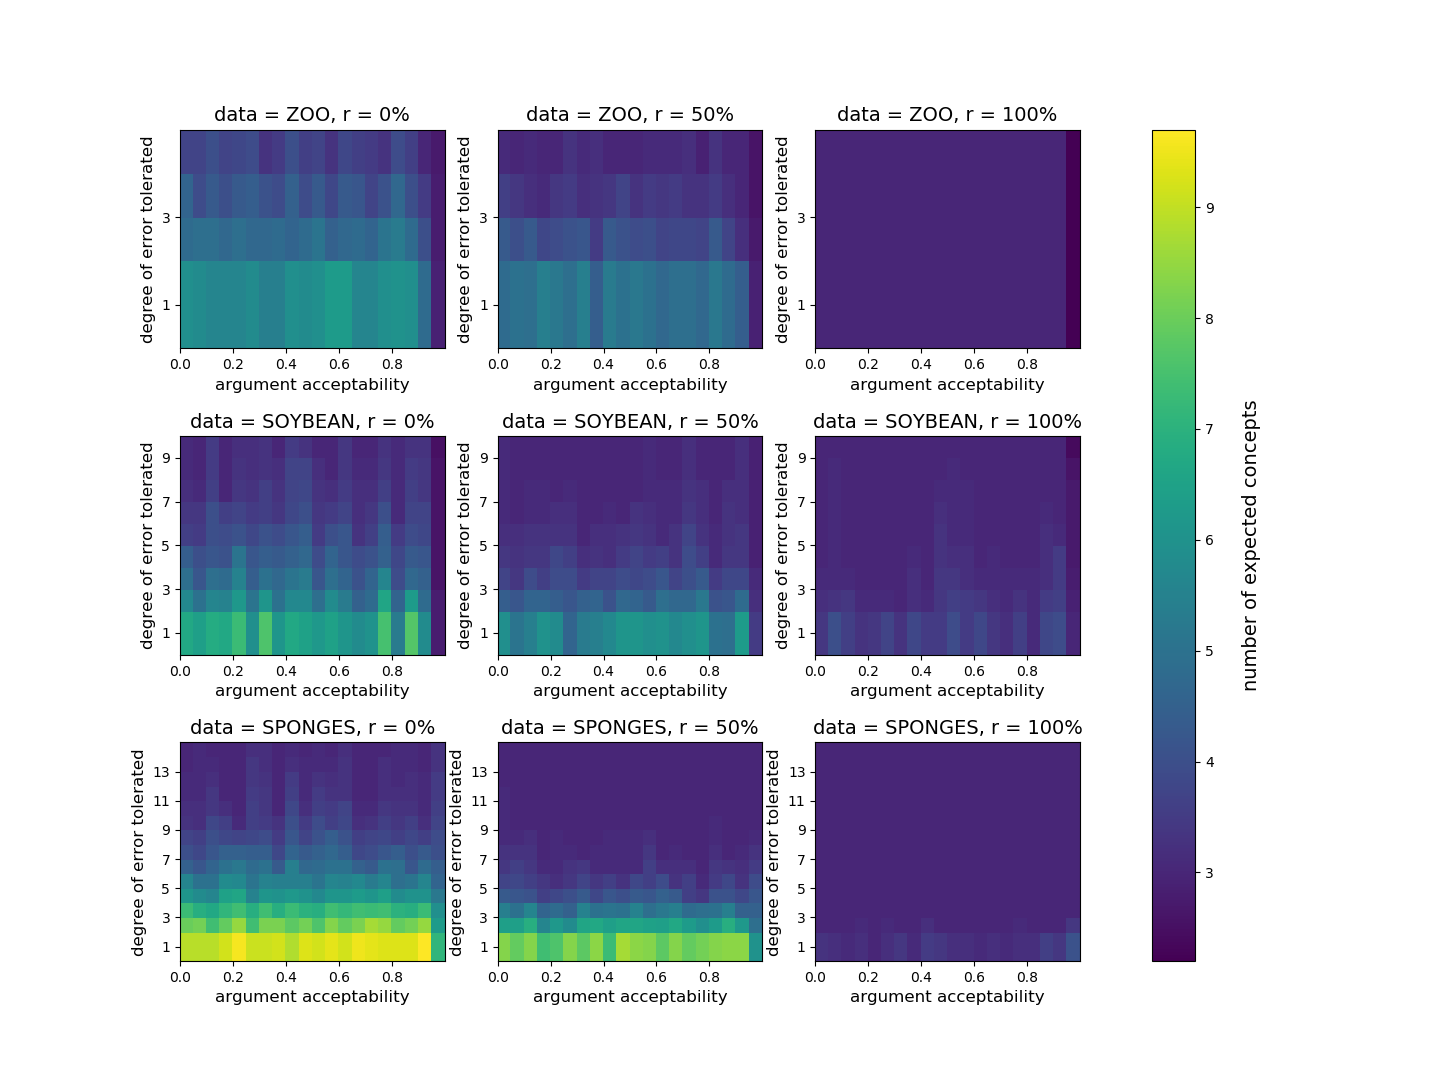
\includegraphics[width = \textwidth]{figs/Figure_parameters.png}
    \caption{Number of expected concepts for each combination of degree of error tolerated $\tau_{E}$, redundancy $r$ and argument acceptability, within the data sets Zoology (ZOO), Soybean (SOYBEAN) and Sponges (SPONGES).}
    \label{fig:param}
\end{figure}

The first thing to observe is that a low percentage of redundancy produces a number of expected concepts closer to three. If the agents start with the same examples in their contexts, they create generalizations that are more likely to correspond to the canonical cases already described in the Chapter \ref{Examples}. While this eases the argumentation, we want to test our argumentation protocol in the worst case of redundancy scenario and therefore, the redundancy parameter will always be set to $100 \%$ in our experiments

With a redundancy set at $100 \%$, we observe that the number of expected concepts depends mostly on the degree of error tolerated, regardless of the data set. With a low degree of error tolerated, we obtain too much concepts as the agents learn over-fit intensional definitions for their concepts. We clearly see that this issue peaks with the Sponges data set, where the number of expected concepts peaks over 9 for an error degree of 1. The lowest degree of error that provides consistently a number of expected concepts close to 3 depends on the data set observed: while $\tau_{E} = 5$ is already satisfying for the Zoology and the Soybean data set, $\tau_{E} = 8$ is a minimum for the Soybean data set.

\begin{figure}[t]
    \centering
    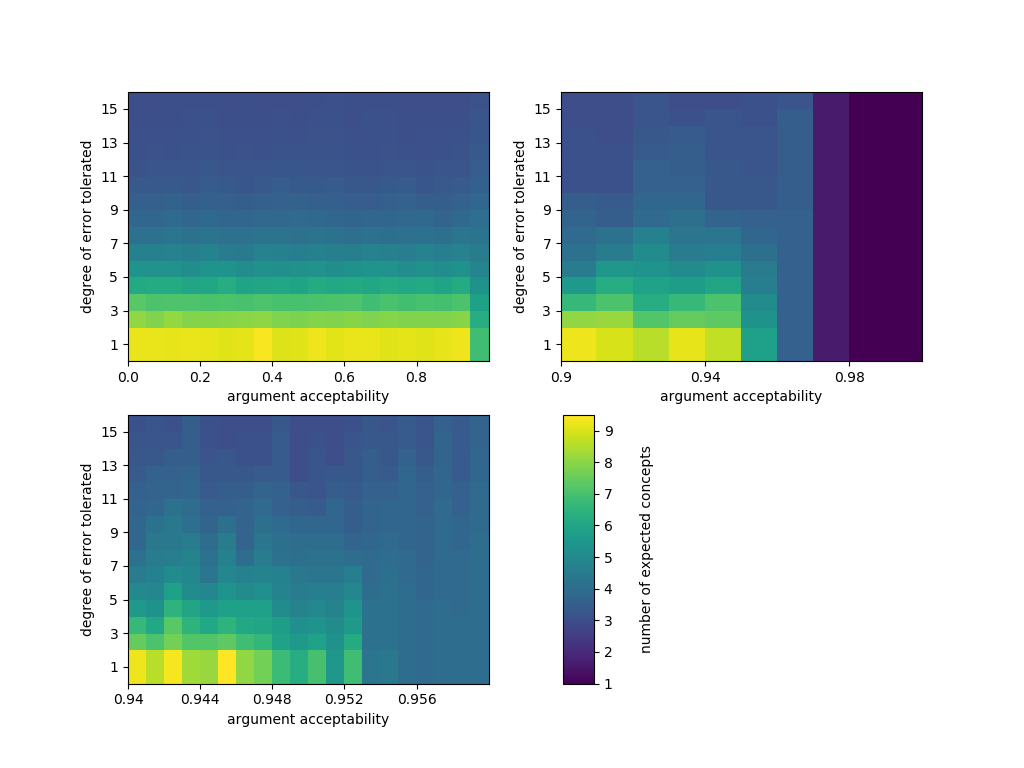
\includegraphics[width = \textwidth]{figs/Figure_AA.png}
    \caption{Impact of argument acceptability on the number of expected concepts on the Sponges data set and for a redundancy of $100\%$ between the two agents' data sets.}
    \label{fig:aa}
\end{figure}

Finally, the argument acceptability does not seems to impact the number of expected concepts, at the exception of its highest values. For each combination of data set, redundancy and degree of error, we can observe a constant number of expected concept until the argument acceptability reaches 0.95, where the number of expected concepts drops drastically, often to 0. The Figure \ref{fig:aa} presents the variation of the number of expected concepts with the sponges data set, for a redundancy of $100 \%$ and argument acceptability values close to 0.95. We can see that the argument acceptability does not influence the number of expected concepts under the value of 0.94. In our experiment, we chose an argument acceptability of 0.75 (? explain ABUI reasons), which is below this threshold.

\section{Impact of the error threshold over argumentation on meaning}

\begin{figure}[t]
    \centering
    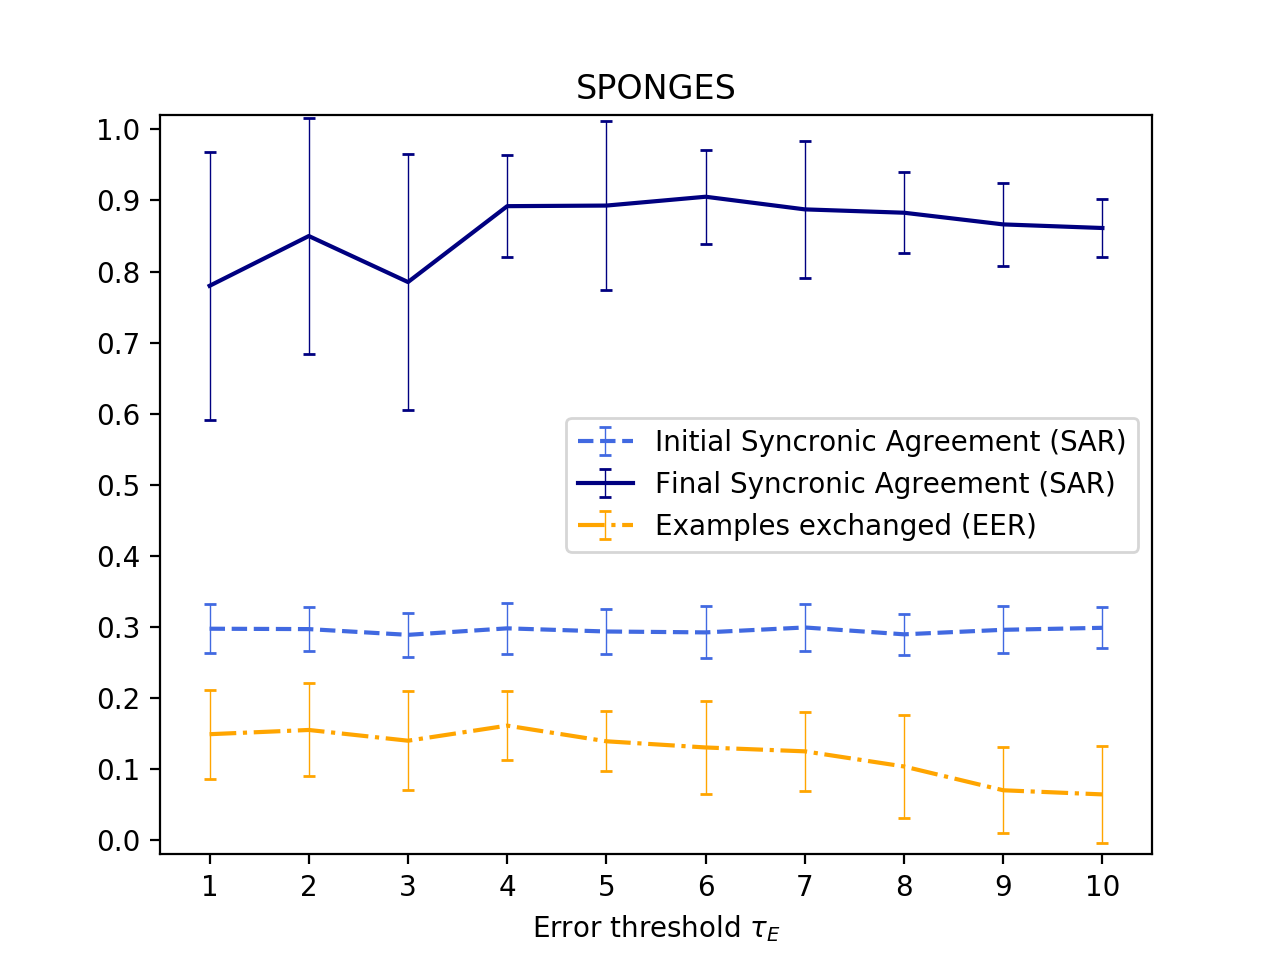
\includegraphics[width = \textwidth]{figs/threshold_SPON.png}
    \caption{Impact of the error threshold on synchronic agreement and examples exchanged, over an argumentation on overlaps in the Sponges data-set.}
    \label{fig:threshold_spon}
\end{figure}

After analyzing the different parameters of our experiments, we observed that the parameter which impacts the most the results of inductive learning is the error threshold. In order to evaluate the impact of the error threshold not only on inductive learning, but on a full argumentation, we are setting up a second experiment in which we measure three dependent variables: the initial synchronic agreement, the final synchronic agreement and the number of exchanged examples. The initial and final synchronic agreement are respectively measured at the beginning and the end of an experiment, using the Synchronic Agreement Ratio or SAR. The SAR is detailed in Section \ref{sec:variables}, and corresponds to the number of examples from the overall context that are named with the same unique sign by both agents divided by the total number of examples in the overall context. The number of exchanged examples is also measured as a ratio, corresponding to the number of examples that have been sent through messages by both agents divided by the total number of examples in the overall context.

The impact of error threshold is tested on two different data-sets: Sponges and Soybeans. For each data-set, we set the argument-acceptability to 0.75 and the redundancy to $0\%$. The error degrees tested vary from one to ten for the Sponges data-set, and from one to fifteen for the Soybean data-set. This difference is based on the comparative sizes of each data-set categories. The argumentation follows a systematic strategy over a setup of as many overlap as the threshold allows.Recall that in order to setup one overlap we need three categories of the data-set, and that in order to use a category of the data-set the number of examples in that category should not be lesser than twice the error threshold. This results in a major difference between the experiments on the two data-sets: while the Sponges data-set is limited to one overlap using any combination of its three 40-examples concepts regardless of the error threshold, the number of overlap increases as the error threshold decreases with the Soybeans data-set since the 19 categories have different numbers of concepts. The systematic strategy and the overlap setup are privileged as they correspond to a baseline setup: the lazy strategy is an adaptation of the systematic strategy, while the overlap setup creates two hypo/hypernymies and a synonymy as well, covering most of the disagreement cases.

\begin{figure}[t]
    \centering
    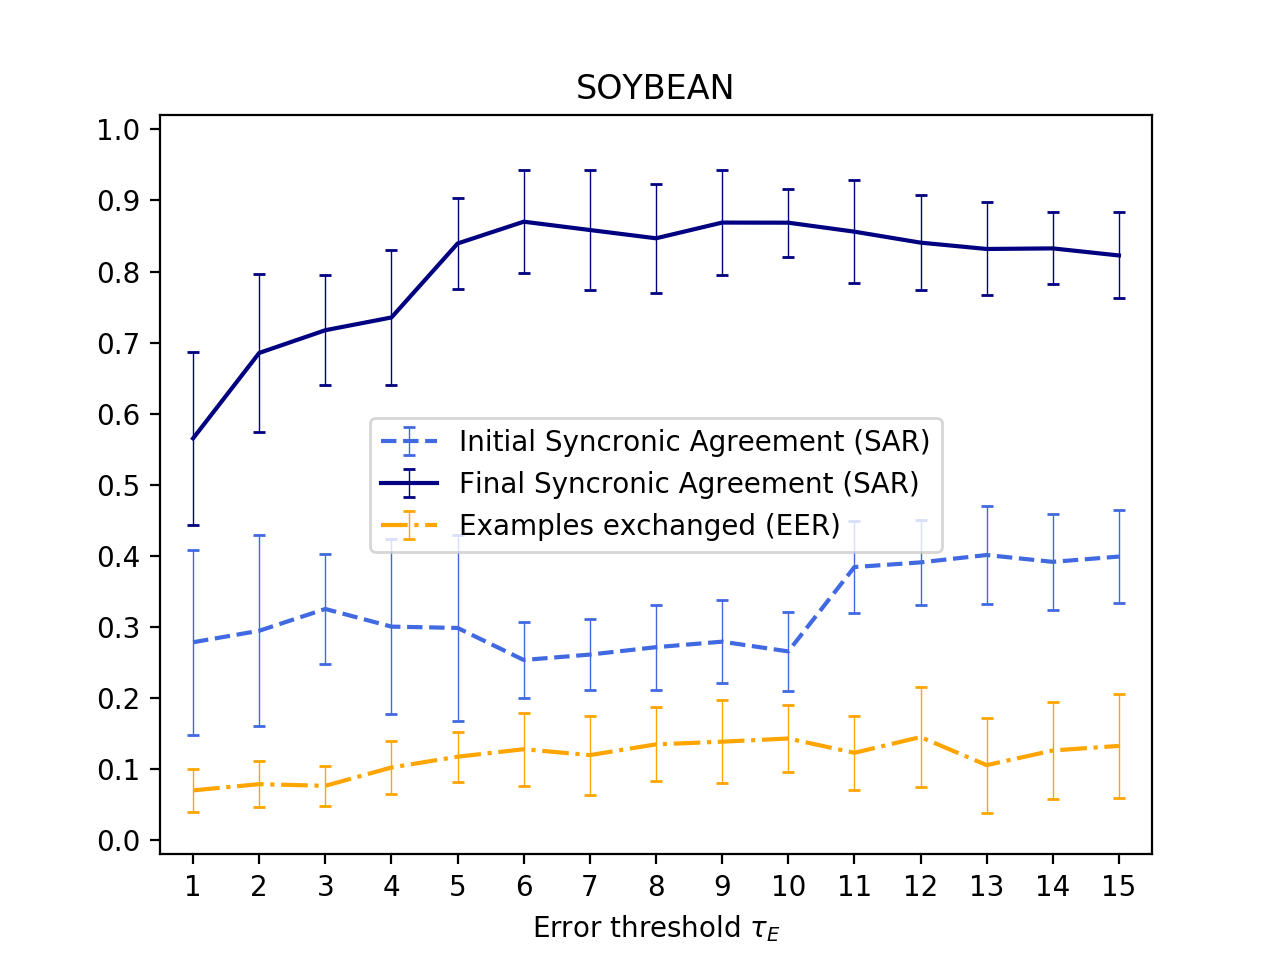
\includegraphics[width = \textwidth]{figs/threshold_SOY.png}
    \caption{Impact of the error threshold on synchronic agreement and examples exchanged, over an argumentation on overlaps in the Soybean data-set.}
    \label{fig:threshold_soy}
\end{figure}

For each data-set, we test the argumentation 500 times with a threshold randomly selected from the data-set dependent range presented in the previous paragraph. Figures \ref{fig:threshold_spon} and show, for each error threshold in absciss, the average initial and final synchronic agreement ratios and the average ratio of exchanged examples in ordinate, along with their standard deviations.

We observe that in both cases, the final synchronic agreement follows a same pattern: initially starting low with a great standard error, it stabilizes above 0.8 once the threshold reaches 5. However, the initial synchronic agreement has a significantly different profile for the two data-sets. With the sponges data-set, we observe an initial SAR that stays at stable to 0.3 regardless of the threshold with the Sponges data-set -- which is expected in a scenario of three concepts of the same size set up in an overlap, as it corresponds to one of the three initial concepts being the intersection of the two overlapping synonyms. On the contrary, the initial SAR in the Soybeans data-set displays multiple increasing and decreasing phases while the threshold varies, as the the threshold allows more or less classes of the data-set in the setup. For instance while we observe an initial SAR at 0.3 for a threshold ranging from 6 to 10, which corresponds to six usable concepts and therefore all of them involved in an overlap, the initial SAR rises at 0.4 above a threshold of 10 as only four concepts remains available for the overlap setup, three of them being used and the last one not causing significant disagreements to impact the initial SAR.

Finally, the number of examples exchanged is also impacted by the choice of the data-set. While the number of exchanged concepts decreases with the error threshold increasing in the Sponges data-set, it increases in the Soybean data-set -- although not by a lot, and mostly when the threshold increases from one to five. A good explanation for this are the poor performances of the argumentation for thresholds ranging on the same values: on that range, the final SAR is significantly below what it is for the same thresholds in the case of Sponges. The inability to generalize, thus not creating good intensional definitions for small concepts and stopping the argumentation early limits the exchange of examples.